\documentclass[a4paper]{article}
\usepackage[latin1]{inputenc}
\usepackage[T1]{fontenc}
\usepackage{graphicx}
\usepackage{amsmath}
\usepackage{hyperref}
\usepackage{listings} %Per inserire codice
\graphicspath{{img/}}
\author{Simone Gasperoni}
\title{Application of Q-Learning to the problem of shortest paths}

\begin{document}

\begin{titlepage}
\begin{center}

\textsc{Machine Learning thesis}\\[0.5cm]
\textsc{MSc in Control Engineering, University of Rome "Sapienza"}\\[0.5cm]

\hrulefill

{ \huge \bfseries Application of Q-Learning to the problem of shortest paths \\[0.4cm] }
\textsc{\Large Simone Gasperoni}\\[0.5cm]
\vfill
\LaTeX

\today

Rome, Italy
\end{center}
\end{titlepage}


\maketitle
\tableofcontents
\newpage

\section{Abstract}
The problem consist in a robot (mono agent) that has to find the shortest route to get to a specific destination (for example in a domestic environment), the agent (robot) uses unsupervised training to learn an unknown environment.
Therefore we face a typical problem of Reinforcement learning.
I decided to implement two versions of Q-Learning (WATKINS, 1989), a traditional and strengthened to improve convergence with the support of a stack (data structure). In fact we can improve convergence  updating the Q-fuction selecting the state-action transitions in reverse chronological order, for each episode from last state to the first state of the episode; see paragraph 13.3.6 of the book by Mitchell.

The java project is here:

\url{https://dl.dropboxusercontent.com/u/59624013/MLproject.zip}
\section{A brief introduction}
\subsection{Reinforcement learning}
In some applications, the output of the system is a sequence of actions. In such a case, a single action is not important; what is important is the policy that is the sequence of correct actions to reach the goal.
Reinforcement learning is the problem of getting an agent to act in the world so as to maximize its rewards. For example, consider teaching a dog a new trick: you cannot tell it what to do, but you can reward/punish it if it does the right/wrong thing. It has to figure out what it did that made it get the reward/punishment, which is known as the credit assignment problem. We can use a similar method to train computers to do many tasks, such as playing backgammon or chess, scheduling jobs, and controlling robot limbs.
\footnote{Kevin Murphy, 1998}
An example of reinforcement learning could be a robot navigating in an environment in search of a goal location. At any time, the robot can move in one of a number of directions. After a number of trial runs, it should learn the correct sequence of actions to reach to the goal state
from an initial state, doing this as quickly as possible and without hitting any of the obstacles.
\footnote{Ethem Alpaydin, 2010}
\begin{figure}[htbp]
\begin{center}
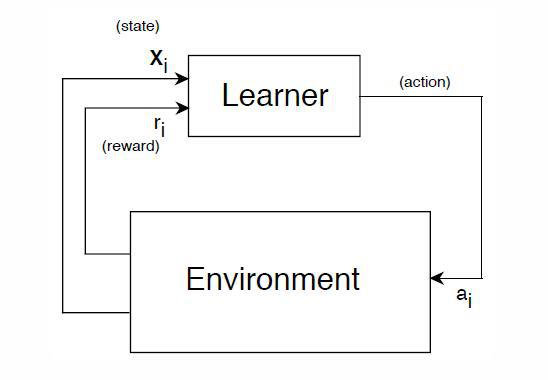
\includegraphics[scale=0.5]{abstract.jpg}
\caption{Reinforcement learning scheme}
\end{center}
\end{figure}
\subsection{Q-Learning}
Q-learning can be used to find an optimal action-selection policy for any given (finite) Markov decision process (MDP). It works by learning an action-value function. When such an action-value function is learned, the optimal policy can be constructed by simply selecting the action with the highest value in each state.

The agent's task is to learn a control policy:
\begin{equation}
\pi : S \rightarrow A
\end{equation}
that maximizes the expected sum of these rewards, with future rewards discounted exponentially by their delay.
\begin{equation}
\ r_{0}+\gamma\cdot r_{1}+\gamma^{2}\cdot r_{2}+ ... +\gamma^{n}\cdot r_{n}
\end{equation}
We call gamma "discount factor" and r "reward". 
The gamma parameter has a range of 0 to 1 (0 <= gamma > 1). If gamma is closer to zero, the agent will tend to consider only immediate rewards. If gamma is closer to one, the agent will consider future rewards with greater weight.

Now we consider this new form of reward:
\begin{equation}
\ V^{\pi}(S)=r_{0}+\gamma\cdot r_{1}+\gamma^{2}\cdot r_{2}+ ... +\gamma^{n}\cdot r_{n}
\end{equation}
that we will call "cumulative reward". To this point we can define an "optimal policy":
\begin{equation}
\pi^{*}(S)=max[ V^{\pi}(S)], \forall s \in S
\end{equation}
\begin{equation}
\pi^{*}(S)=max[ r_{0}+\gamma\cdot r_{1}+\gamma^{2}\cdot r_{2}+ ... +\gamma^{n}\cdot r_{n}]
\end{equation}
Of course the agent's policy must choose among actions, not among states:
\begin{equation}
\pi^{*}(S)=max[ r(s,a)+ \gamma V^{*}(\delta (s,a))]
\end{equation}
Let us define the evaluation function Q(s,a) so that its value is the maximum discounted cumulative reward that can be achieved starting from state s and applying action a as the first action. In other words, the value of Q is the reward received immediately upon executing action 'a' from state 's', plus the value (discounted by gamma) of following the optimal policy thereafter.
\begin{equation}
Q(s, a)=r(s, a) + \gamma V^{*}(\delta (s,a))
\end{equation}
\begin{equation}
\pi^{*}(S)=max[Q(s,a)]
\end{equation}
This rewrite shows that if the agent learns the Q function instead of the V function, it will be able to select optimal actions even when it has no knowledge of the function r and delta

Finally the transition rule of Q learning is a very simple formula:
\begin{equation}
Q(s, a)=r(s, a)+ \gamma*max[Q(\delta(s,a), a')]
\end{equation}
being
\begin{equation}
V^{*}(s)=max[Q(s, a')]
\end{equation}

The equation number 9 is a recursive definition of Q, this definition provides the basis of algorithm that iteratively approximate Q (WATKINS 1989).
\begin{verbatim}
The Q-Learning algorithm goes as follows:

    1. Set the gamma parameter, and environment rewards in matrix R.

    2. Initialize matrix Q to zero.

    3. For each episode:

        Select a random initial state.

        Do While the goal state hasn't been reached.

            Select one among all possible actions for the current state.
            Using this possible action, consider going to the next state.
            Get maximum Q value for this next state based on all possible actions.
            Compute: Q(state, action) = 
               R(state, action) + gamma * Max[Q(next state, all actions)]
            Set the next state as the current state.

        End Do

    End For
\end{verbatim}
\newpage
\section{The problem and the design choices}
\subsection{The problem}
We can imagine that the destination is a room or an exit door, each room had an index to denote unambiguously a corresponding state as shown in the Figure 2 below:
\begin{figure}[htbp]
\begin{center}
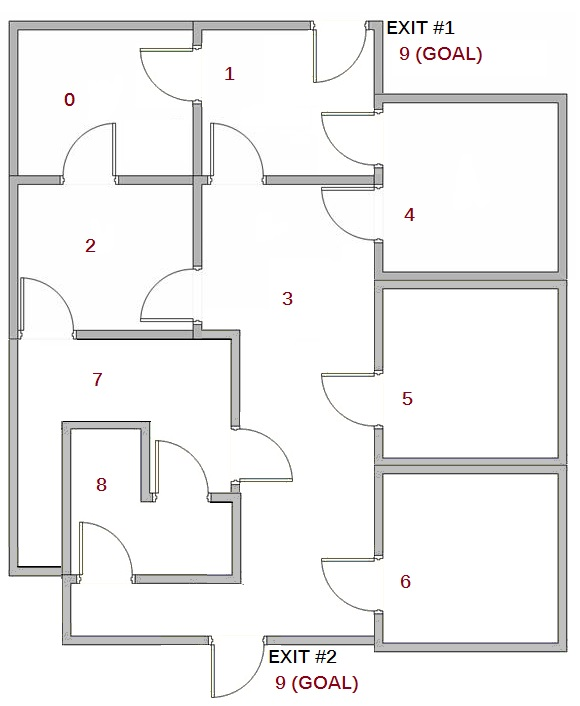
\includegraphics[scale=0.5]{problem2.jpg}
\caption{House with indexed rooms}
\end{center}
\end{figure}

Moreover, as can be seen, when the robot is out of the house is still in a indexed state (which in this case is the GOAL-STATE). 
Our virtual agent will learn through experience, without a teacher (this is called unsupervised learning).  The agent will explore from state to state until it reaches the goal. We'll call each exploration an episode.  Each episode consists of the agent moving from the initial state to the goal state.  Each time the agent arrives at the goal state, the program goes to the next episode.

As we shall see later, the environment is modeled with a deterministic Markov decision process, in which the states (S) are the rooms, and the actions (A) are the possible movements among the rooms.
In the next subsection I will introduce the design choices made for represent the environment on which the Q-Learning algorithm will find the shortest paths to reach the goal state.

\subsection{Exploit/explore dilemma}
One obvious strategy would be for the agent in state s is to select the action a that maximizes Q(s, a), thereby exploiting its current approximation Q. However with this strategy the agent runs the risk that it will overcommit to actions that are found during early trainig to have high Q values, while failing to explore other actions that have even higher value.

\textbf{My choice is to divide episodes into two parts: the first part with a strategy of pure exploration and a second part with a strategy of pure exploitation.}

NOTE: EPISODES=episodesExploring+episodesExploiting

\begin{lstlisting}[caption={Java code}]
for(int j = 0; j < episodesExploring; j++){
     episodeExploringWithStack(new Random().nextInt(qSize));
}
for(int j = 0; j < episodesExploiting; j++){
     episodeExploitingWithStack(new Random().nextInt(qSize));
}
\end{lstlisting}


\subsection{Environment}
Markov decision processes formally describes an environment for Reinforcement learning, where the environment is fully observable.

A Markov decision process is a 4-tuple:

\begin{equation}
Mdp=<S, A, \delta(s,a), r(s,a)>
\end{equation}
Where:
\begin{itemize}
  \item actions set is \begin{displaymath} A \end{displaymath}
  \item states set is \begin{displaymath} S \end{displaymath}
  \item transition function is \begin{displaymath} \delta(s,a) \end{displaymath}
  \item reward function is \begin{displaymath} r(s,a) \end{displaymath}
\end{itemize}

The markovian model for domestic environment in Figure 2 can be represented as the following graph.
\begin{figure}[htbp]
\begin{center}
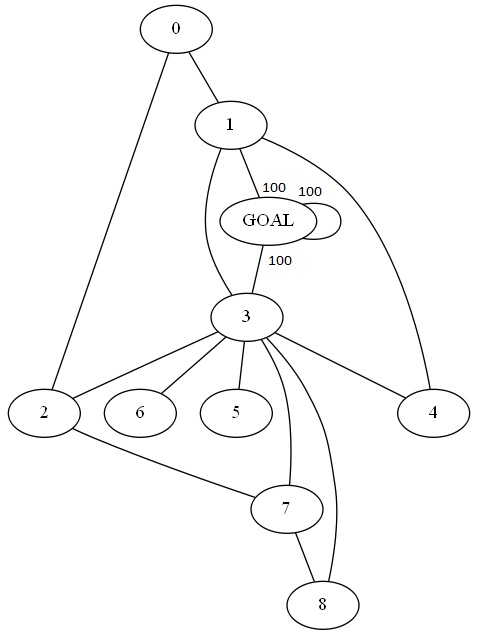
\includegraphics[scale=0.5]{graph.jpg}
\caption{Graph, states and transitions of environment}
\end{center}
\end{figure}

I hypothesize that the topology of the environment is given to the agent as the R matrix. 
In fact as we can see in the Formula 12 matrix R (rewards matrix) describes exactly the environment, considering that the -1's in the table represent there isn't a link between nodes, whereas the goal state is indicated with a prize of 100, with all other awards 0 (possible transition state=state*action).
The columns of R represent the actions from 0 to n, whereas the rows represent the states from 0 to n.
In addition hypothesized that the matrix R is independent of time having to represent a static environment, finally, the environment is deterministic because each transition leads to only one destination state.

\begin{equation}
R= \begin{bmatrix}
$$
-1 & 0 & 0 & -1 & -1 & -1 & -1 & -1 & -1 & -1 \\
0 & -1 & -1 & 0 & 0 & -1 & -1 & -1 & -1 & 100 \\
0 & -1 & -1 & 0 & -1 & -1 & -1 & 0 & -1 & -1 \\
-1 & 0 & 0 & -1 & 0 & 0 & 0 & 0 & 0 & 100 \\
-1 & 0 & -1 & 0 & -1 & -1 & -1 & -1 & -1 & -1 \\
-1 & -1 & -1 & 0 & -1 & -1 & -1 & -1 & -1 & -1 \\
-1 & -1 & -1 & 0 & -1 & -1 & -1 & -1 & -1 & -1 \\
-1 & -1 & 0 & 0 & -1 & -1 & -1 & -1 & 0 & -1 \\
-1 & -1 & -1 & 0 & -1 & -1 & -1 & 0 & -1 & -1 \\
-1 & 0 & -1 & 0 & -1 & -1 & -1 & -1 & -1 & 100
$$
\end{bmatrix}
\end{equation}
\newpage

\section{Testing and evaluation of performance}

For the evaluation of performance I have considered 5 parameters:

\textbf{Gamma}: discount factor.

\textbf{Episodes}: number of episodes in EXPLORATION and EXPLOITATION.

\textbf{Step}: number of step after the learning stage.

\textbf{State}: number of states visited during the learning stage.

\textbf{Time}: duration of the learning stage measured in msec, this is an important attribute, especially in emergency situations where time is more important than absolute convergence to the optimum condition (see firefighter robot).

The measure of the results is obtained with Java method void test(), it measures the lenghts of paths to goal state starting from every state and taking the average of the lengths of paths.

Follow the Java test method:
\begin{verbatim}
public double test(){
    int state=0;
    for(int i = 0; i<qSize; i++){
       	state=i;
       	System.out.println("");
       	while(state!=qSize-1){
    	    state=getMaximumNextAction(state);
    	    System.out.print(" | "+state);
    	    step++;
        }
      	System.out.println("");
    }
    return (double)step/qSize;
} 
\end{verbatim}
\textbf{We will see how the version WITHSTACK increases the learning time, reduces the number of states visited in learning stage, massively increases RAM usage, and improves the convergence conditions optimal with respect to the number of episodes.}
\newpage
\subsection{Convergence environment 1}
\begin{figure}[htbp]
\begin{center}
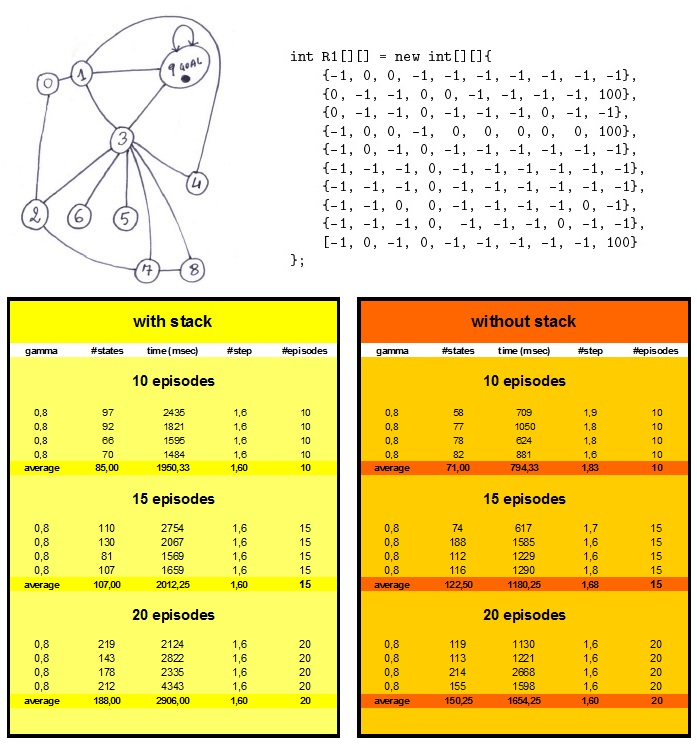
\includegraphics[scale=0.75]{env1.jpg}
\caption{Environment}
\end{center}
\end{figure}
I decided to set half episodes in EXPLORATION and half in EXPLOTATION.
On average the best route employs 1.6 step. 
Unfortunately this environment is very connected, in this environment we don't appreciate the improvement made by the stack data structure about the convergence to optimal condition.
We can note that the version with stack converges to the optimal condition (number of steps = 1.6) in only 10 episodes whereas the "without stack version" needs of about 20 episodes.
On the other hand, the "without stack version" is faster than other version, the cause is that the "without stack version" doesn't manage auxiliary data structure during the learning stage, is thereby more fast.

\subsection{Convergence environment 2}
\begin{figure}[htbp]
\begin{center}
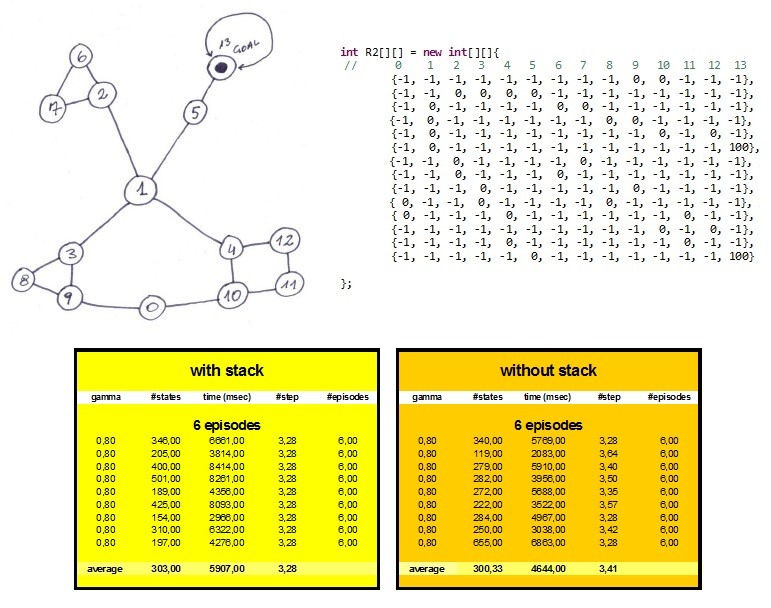
\includegraphics[scale=0.75]{env2.jpg}
\caption{Environment}
\end{center}
\end{figure}
I decided to set five episodes in EXPLORATION and the last episode in EXPLOITATION.
The result is the same of the other environment but the trends are more visible because the graph is less connected than other.

\newpage
\section{Implementation of the episodes in Java code}
\subsection{method train(mode)}
\begin{verbatim}
...
    //enum mode = 'WITHSTACK' or 'WITHOUTSTACK'
    public long train(mode e){             
    	long time=0;
    	long endTime=0;
    	//episodes with stack:
    	if(e==mode.WITHSTACK){
    	    time = System.nanoTime();
    	    for(int j = 0; j < episodesExploring; j++){
                episodeExploringWithStack(new Random().nextInt(qSize));
            }
    	    for(int j = 0; j < episodesExploiting; j++){
                episodeExploitingWithStack(new Random().nextInt(qSize));
            }
            endTime = System.nanoTime()-time; 
    	}
    	//episodes without stack
    	if(e==mode.WITHOUTSTACK){
     	    time = System.nanoTime();
     	    for(int j = 0; j < episodesExploring; j++){
                episodeExploringWithoutStack(new Random().nextInt(qSize));
             }
     	     for(int j = 0; j < episodesExploiting; j++){
                episodeExploitingWithoutStack(new Random().nextInt(qSize));
             }
             endTime = System.nanoTime()-time; 
     	}
    	//PRINT THE Q-FUNCTION
        System.out.println("q[i][j] values:");
        for(int i = 0; i < qSize; i++){
             for(int j = 0; j < qSize; j++){
                 System.out.print(q[i][j] + ",\t");
             } 
             System.out.print("\n");
        }
        System.out.print("\n");
        return endTime;
    }
...
\end{verbatim}
\newpage
\subsection{WITHSTACK episode}
\begin{verbatim}
...
    private void episodeExploringWithStack(int initialState){
   	    currentState = initialState;
        //I hypothesize that the goal state is always the last (qSize-1)
        //Travel from state to state until goal state is reached
        while(currentState!=qSize-1){
     	   statesStack.push(currentState);
     	   currentState=getRandomAction();
     	   actionsStack.push(currentState);
           counter++;
        }
        while(!statesStack.isEmpty()){
     	   int state=statesStack.pop();
     	   int action=actionsStack.pop();
     	   if(R[state][action]>=0){
q[state][action]=(int)(R[state][action]+(gamma*maximum(action)));
           }   
        }
    }   
    private void episodeExploitingWithStack(int initialState){
    	currentState = initialState;
        //I hypothesize that the goal state is always the last (qSize-1)
        //Travel from state to state until goal state is reached
        while(currentState!=qSize-1){
           statesStack.push(currentState);
           currentState=getMaximumNextAction(currentState);
           actionsStack.push(currentState);
           counter++;
        }
        while(!statesStack.isEmpty()){
           int state=statesStack.pop();
           int action=actionsStack.pop();
           if(R[state][action]>=0){
q[state][action]=(int)(R[state][action]+(gamma*maximum(action)));
           }   
        } 
    }
...
\end{verbatim}
\newpage
\subsection{WITHOUTSTACK episode}
\begin{verbatim}
...
    private void episodeExploringWithoutStack(int initialState){
        currentState = initialState;
        //I hypothesize that the goal state is always the last (qSize-1)
        //Travel from state to state until goal state is reached
        while(currentState!=qSize-1){
           int possibleAction = 0;
           possibleAction = getRandomAction();
           if(R[currentState][possibleAction]>=0){
              q[currentState][possibleAction]=
(int)(R[currentState][possibleAction] + (gamma * maximum(possibleAction)));
              currentState = possibleAction;
           }
           counter++;
        }  
    }  
    private void episodeExploitingWithoutStack(int initialState){
        currentState = initialState;
        //I hypothesize that the goal state is always the last (qSize-1)
        //Travel from state to state until goal state is reached
        while(currentState!=qSize-1){
            int possibleAction = 0;
            possibleAction = getMaximumNextAction(currentState);
            if(R[currentState][possibleAction]>=0){
                q[currentState][possibleAction]=
(int)(R[currentState][possibleAction] + (gamma * maximum(possibleAction)));
                currentState = possibleAction;
            }
            counter++;
        }  
    }
...

\end{verbatim}
\section{References}
References and bibliography
 
  Mitchell Machine Learning - Mc Graw-Hill (International edition, 1997)
 
  Machine Learning lecture notes and slides, Sapienza University of Rome
 
  Alpaydin Introduction to Machine Learning (Second edition, 2010)

  Kevin Murphy, 1998

  http://en.wikipedia.org/

  http://mnemstudio.org/
\end{document}